
%\begin{wrapfigure}[0.5]{R}{0.5\textwidth}
\begin{figure*}[t]\centering%
	%\scalebox{0.9}{\small\input{pics/diagram-20220513}}%overallApproach}}
	%\vspace*{-0.3cm}
	\centering
	%	\hspace{-0.9cm}
	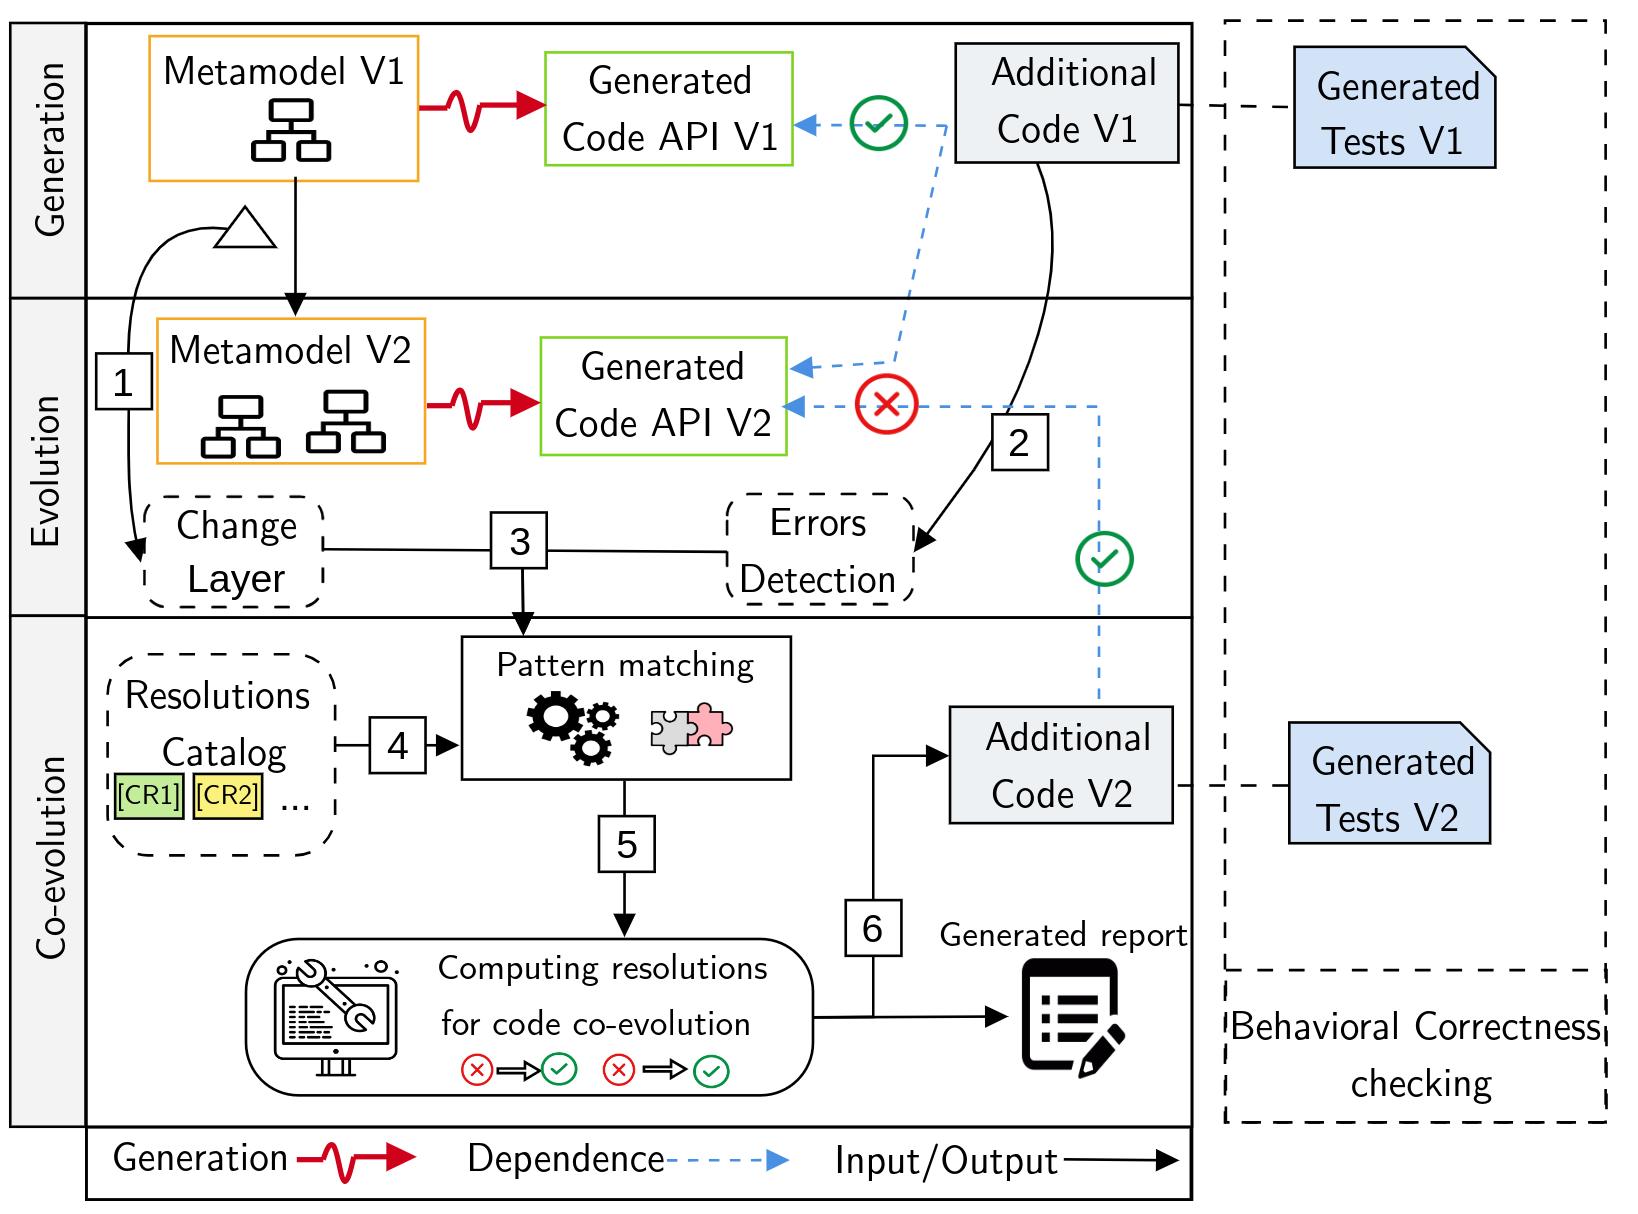
\includegraphics[width=0.8\textwidth]{./pics/chapter1pics/ApproachV5.png}
	\caption{Overall approach for metamodel and code co-evolution}
	\label{fig:overallapproach}
	%\vspace{-1em}
	\vspace{-1em}
\end{figure*}
%\end{wrapfigure}
%\section{Change detection}
\label{sec: ap1_changedetection}

\section{Motivating Example}\label{example}

This section introduces a motivating example to illustrate the challenge of metamodel and code co-evolution. 
Let us take as an example the Modisco project \cite{MDTModisco}, which has evolved numerous times in the past. Modisco is an academic initiative project implemented in the Eclipse platform to support the development of model-driven tools, reverse engineering, verification, and transformation of existing software systems \cite{bruneliere2010modisco,bruneliere2014modisco}.


Figure \ref{fig: BMM} shows an excerpt of the "Modisco Discovery Benchmark" metamodel\footnote{\url{https://git.eclipse.org/r/plugins/gitiles/modisco/org.eclipse.modisco/+/refs/tags/0.12.1/org.eclipse.modisco.infra.discovery.benchmark/model/benchmark.ecore}} consisting of 10 classes in version~0.9.0.
It illustrates some of the domain concepts \textbf{Discovery}, \textbf{Project}, and \textbf{ProjectDiscovery}  used for the discovery and reverse engineering of an existing software system. 
From these metaclasses, a first code API is generated, containing Java interfaces and their implementation classes, a factory, a package, etc. Listing \ref{lis:Modisco_Code_API_V1} shows a snippet of the generated Java interfaces and classes from the metamodel in Figure \ref{fig: BMM}. 

The generated code API is further enriched by the developers with additional code functionalities in the "Modisco Discovery Benchmark" project and its dependent projects as well.
For instance, by implementing the methods defined in metaclasses and advanced functionalities in new classes. Listing \ref{lis:Modisco_Code_External_V1} shows the two classes \texttt{Report} and \texttt{CDOProjectDiscoveryImpl} of the additional code in the same project "Modisco Dsicovery Benchmark" and in another dependent project, namely the "Modisco Java Discoverer Benchmark" project. 
In version~0.11.0, the "Modisco Discovery Benchmark" metamodel evolved with several significant changes, among which the following impacting changes:

\begin{enumerate}%[noitemsep,nolistsep]
	
	\item Deleting the metaclass \texttt{ProjectDiscovery}. 
	
	\item Renaming the property \emph{totalExecutionTimeInSeconds} to \emph{discoveryTimeInSeconds} in metaclass \texttt{Discovery}. 
	
	\item Moving the property \emph{discoveryTimeInSeconds} (after its rename) from metaclass \texttt{Discovery} to \texttt{DiscoveryIteration}. 
	
\end{enumerate} 


\begin{figure}
	
	\centering
	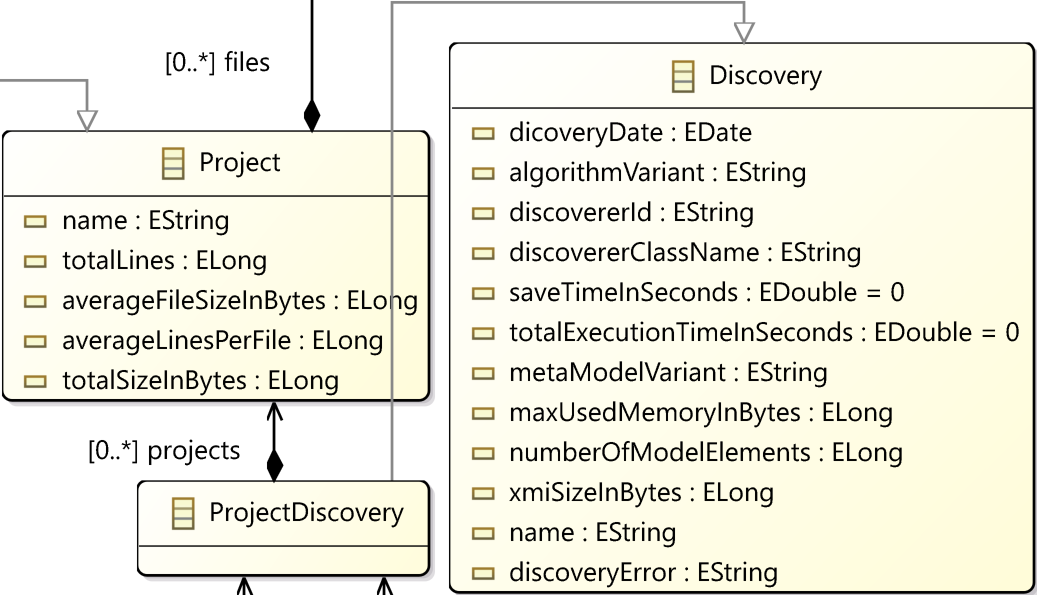
\includegraphics[width=0.48\textwidth]{pics/chapter1pics/example.PNG}
	\caption{Excerpt of Modisco Benchmark metamodel in version 0.9.0.}
	\label{fig: BMM}
	\vspace{-5mm}
\end{figure}

After applying these metamodel changes, naturally, the code of Listing \ref{lis:Modisco_Code_API_V1} is regenerated from the evolved version of the metamodel, which in turn impacts the existing additional code depicted in Listings \ref{lis:Modisco_Code_External_V1}. 
The resulting errors in the original code in version 0.9.0 are underlined in red in Listing \ref{lis:Modisco_Code_External_V1}. 
Listing \ref{lis:Modisco_Code_External_V2} presents the final result of the co-evolution process in version 0.11.0. The co-evolved code is underlined in green. 
For example, in response to the \textit{delete} of the metaclass \texttt{ProjectDiscovery}, its import statement {\small\boxed{Line~1}} in Listing \ref{lis:Modisco_Code_External_V1}, and any usage of it or its methods are impacted. The import statement is completely removed. The same can be applied to the usages of the class and its methods. Alternatively, they could also be replaced by a default value rather than removing the whole instruction. The intention is to maintain the developers' code with minimal removal co-evolution. 

Furthermore, the same changes \textit{rename} and \textit{move} of the property \emph{totalExecutionTimeInSeconds} impact two usages that are co-evolved differently. First, the call of \texttt{setTotalExecutionTimeInSeconds} ({\small\boxed{Line~4}} in Listing~\ref{lis:Modisco_Code_External_V1}) that is co-evolved by renaming it to \texttt{setDiscoveryTimeInSeconds}, then extending the path with \texttt{getIterations()}. The second impact is the use of the generated literal \texttt{BenchmarkPackage.}\emph{\footnotesize{DISCOVERY\_\_TOTAL\_EXECUTION\_TIME\_IN\_SECONDS}}. It is successively co-evolved by renaming it to \texttt{BenchmarkPackage.}\emph{\footnotesize{DISCOVERY\_\_DISCOVERY\_TIME\_IN\_SECONDS}} before replacing its source class \texttt{DISCOVERY} by \texttt{DISCOVERY\_ITERATION}. 
Note that when using the IDE quick fixes to co-evolve these errors, it suggests to create the method \texttt{setTotalExecutionTimeInSeconds} in the class \texttt{Discovery} and the literal \emph{\footnotesize{DISCOVERY\_\_TOTAL\_EXECUTION\_TIME\_IN\_SECONDS}} in the class \texttt{BenchmarkPackage}, which does not meet the required co-evolutions shown in Listing~\ref{lis:Modisco_Code_External_V2}.

The above examples show the importance of correctly matching the different code usages and patterns of the generated code elements with the metamodel evolution changes to co-evolve them with the appropriate resolutions. 

The next section presents our contribution for a fully automatic co-evolution of metamodel and code.  

\begin{lstlisting}[language=Java,breaklines=true,mathescape,literate={\-}{}{0\discretionary{-}{}{}},caption=excertprpt of the generated code in org.eclipse.modisco.infra.discovery.benchmark.\label{lis:Modisco_Code_API_V1}]
	//Discovery Interface
	public interface Discovery extends EObject {
		double getTotalExecutionTimeInSeconds();
		void setTotalExecutionTimeInSeconds(double value);
		...
	}
	//Project Interface
	public interface ProjectDiscovery extends Discovery {...}
	//DiscoveryImpl Class
	public class DiscoveryImpl extends EObjectImpl implements Discovery {
		public double getTotalExecutionTimeInSeconds() {...}
		public void setTotalExecutionTimeInSeconds(double totalExecTime) {...}
		...
	}
\end{lstlisting}
%xleftmargin=0.2cm,xrightmargin=0cm,framexleftmargin=+6pt,frame=single,
\begin{lstlisting}[language=Java,breaklines=true,mathescape,literate={\-}{}{0\discretionary{-}{}{}},caption=Excerpt of the additional code V1.\label{lis:Modisco_Code_External_V1}]
	import (*{\scriptsize org.eclipse.modisco.infra.discovery.benchmark}*).(*\ul{\scriptsize ProjectDiscovery}*);
	public class Report {
		...
		discovery.(*\ul{setTotalExecutionTimeInSeconds}*)(...);
	}
	...
	public class CDOProjectDiscoveryImpl extends AbstractCDODiscoveryImpl implements CDOProjectDiscovery {
		...
		case JavaBenchmarkPackage.
		CDO_PROJECT_DISCOVERY__TOTAL_EXECUTION_TIME_IN_SECONDS: return BenchmarkPackage.
		(*\ul{DISCOVERY\_\_TOTAL\_EXECUTION\_TIME\_IN\_SECONDS}*);
		...
	}
	
	
\end{lstlisting}

\begin{comment}
	public class JavaDiscoveredProjectImpl extends AbstractJavaProjectImpl implements JavaDiscoveredProject {
		
		public int eBaseStructuralFeatureID(int derivedFeatureID, Class<?> baseClass) {
			...
			case JavaBenchmarkPackage.JAVA_DISCOVERED_PROJECT__DISCOVERIES: return BenchmarkPackage.
			(*\ul{DISCOVERED\_PROJECT\_\_DISCOVERIES}*);
			...
		}
		...
	}
\end{comment}
%%%%%%%%%%%%%%%%%%%%%%%%%%%%%%%%%%%%%%%%%%%%%%%%%%%%%%%%%%%
%%                   Now the evolved code                %%
%%%%%%%%%%%%%%%%%%%%%%%%%%%%%%%%%%%%%%%%%%%%%%%%%%%%%%%%%%%
\setulcolor{green} 
\setstcolor{green}
%\setstcolor{green}
%,xleftmargin=0.2cm,,xrightmargin=-0cm,framexleftmargin=+6pt,frame=single
\begin{lstlisting}[language=Java,breaklines=true,mathescape,literate={\-}{}{0\discretionary{-}{}{}},caption=Excerpt of the additional code V2.\label{lis:Modisco_Code_External_V2}]
	(*{\st{import }}*)(*{\scriptsize \st{ org.eclipse.modisco.infra.discovery.benchmark. ProjectDiscovery}}*);
	public class Report {
		...
		discovery.(*\ul{getIterations().}*) 
		(*\ul{setDiscoveryTimeInSeconds}*)(...);
		...
	}
	public class CDOProjectDiscoveryImpl extends AbstractCDODiscoveryImpl implements CDOProjectDiscovery {
		...
		case JavaBenchmarkPackage.
		CDO_PROJECT_DISCOVERY__TOTAL_EXECUTION_TIME_IN_SECONDS: return BenchmarkPackage.
		(*\ul{DISCOVERY\_ITERATION\_\_DISCOVERY\_TIME\_IN\_SECONDS}*);
		...
	}
	...
}
\end{lstlisting}
%\begin{lstlisting}[language=Java,breaklines=true,mathescape,literate={\-}{}{0\discretionary{-}{}{}},xleftmargin=0.2cm,xrightmargin=-0.4cm,framexleftmargin=+6pt,frame=single,caption=Excerpt of the additional external code in the SL org.eclipse.modisco.infra.discovery.benchmark.\label{lis:Modisco_Code_External_V1}]

\begin{comment}
....
public class JavaDiscoveredProjectImpl extends AbstractJavaProjectImpl implements JavaDiscoveredProject {
	public int eBaseStructuralFeatureID(int derivedFeatureID, Class<?> baseClass) {
		...
		case JavaBenchmarkPackage.JAVA_DISCOVERED_PROJECT__DISCOVERIES: return BenchmarkPackage.(*\ul{BENCHMARK\_\_DISCOVERIES}*);
		...
	}
	...
}
\end{comment}



\section{Approach}\label{approach}

This section presents the overall approach of our automated co-evolution of code with evolving metamodels,  instantiating on the Ecore technological space. First, we give an overview of the approach and specify the metamodel evolution changes we consider. 
%
Then, we present how we retrieve the resulting errors due to metamodel evolution, followed by the regeneration of the code API. 
After that, we present the pattern matching process, which is an important part of our fully automatic co-evolution approach, before discussing the resolutions of the code errors. 

\subsection{Overview}
\label{Overview}
Figure~\ref{fig:overallapproach} depicts the overall steps for the automatic co-evolution of the metamodel and code, with horizontally separated parts defining chronological order from the top to the bottom.
%\\
After the generation step (the upper part of Figure~\ref{fig:overallapproach}), the evolution of the Ecore metamodel will cause errors in the additional Java code that depends on the API of the newly generated code (the middle part of Figure~\ref{fig:overallapproach}). We take as input the evolution changes of the metamodel between the two versions of this metamodel {\small\boxed{1}}. Then, we parse the additional code  {\small\boxed{2}} to retrieve the list of errors. 
After that, we get to the bottom part of Figure~\ref{fig:overallapproach}, both the list of metamodel changes and the list of errors are used as inputs for the \red{pattern matching step {\small\boxed{3}}. It analyzes the structure of the error to match it with its impacting metamodel change and decides which resolution  {\small\boxed{4}} to apply for the error co-evolution {\small\boxed{5}}. The metamodel changes provide the ingredients and necessary information that are used for the co-evolution.  
	At the end of the automatic co-evolution, we obtain a new co-evolved additional code {\small\boxed{6}} along a generated report on the applied resolutions.} 
In addition to the automatic co-evolution, we generate test cases before and after co-evolution to highlight its possible effect. In fact, many research papers rely on the use of tests to check the behavior of the code during its evolution. For example, Godefroid et al.~\cite{10.1145/3395363.3397374} uses tests to find regressions in different versions of REST APIs. In particular, Lamothe et al.~\cite{9079197},~\cite{10.1145/3387905.3388608} use tests to validate the evolution of the client code after Android API migration. We apply a similar method to check the effect of the co-evolution. 
Finally, during the co-evolution process, we generate a report linking the applied resolutions for each code error with its impacting metamodel change. If needed, this can help developers in understanding the performed co-evolution, since we fully automate it.
%\todo{refs behavioral check et papier android : to check}
%\DK{we see later if we add the story of generated tests after co-evolution}

\subsection{Metamodel Evolution Changes}
\label{mmchanges}

One of the intrinsic properties of software artifacts is its continuous evolution~\cite{mens2008introduction}. Metamodels are no different and are meant to evolve. 
Two types of evolution changes are considered when evolving a metamodel: \emph{atomic} and \emph{complex} changes~\cite{Herrmannsdoerfer2011}. 
Atomic changes are additions, removals, and updates of a metamodel element. Complex changes consist of a sequence of atomic changes combined together~\cite{vermolen_reconstructing_2012},~\cite{khelladi2015detecting}. For example, move property is a complex change where a property is moved from a source class to a target class. This is composed of two atomic changes: delete property and add property~\cite{Herrmannsdoerfer2011}. 
Many approaches in the literature~\cite{Alter2015, williams2012searching,cicchetti_managing_2009,langer_posteriori_2013,vermolen_reconstructing_2012,Khelladi2016,bettini2022executable} exist to detect metamodel changes between two versions. Note that the detected list of complex changes does not include the list of the detected atomic changes, i.e., no overlap in between. 
\red{Moreover, the detection approaches must order the changes in a consistent way. This is fundamentally a problem that change detection approaches must deal with, and hence, is out of scope for our problem of code co-evolution. Nonetheless, it is important and expect a consistent order of changes to not hinder the quality of the co-evolution.}

For the purpose of modularity and extensibility, we use a specification layer for the changes~{\small\boxed{1}} that is simply a connection layer to our co-evolution approach with existing change detection approaches. This connection layer specifies our own representation of a metamodel change that can be mapped later with any change representation. \red{It simply specifies the needed information for each change in the form of its attributes. In the left column of Table \ref{table:ResolutionsCatalog}, we precise the impacting changes that we consider in our work. For each change, we precise in the second column the attributes that represent and compose each change. When using a state-of-the Art detection approach, we analyze in white box the detected changes to extract their attributes and map them to our internal change layer.
	%the attributes of each change are mapped with the corresponding detected change. In order to map the output changes of the used detection approach, we analyze in white box their results to retrieve their different attributes and map them with our change layer.
} 
For example, a rename property change includes information regarding its old name, new name, and its class container. Therefore, in practice, any detection approach~\cite{Alter2015, williams2012searching,cicchetti_managing_2009,langer_posteriori_2013,vermolen_reconstructing_2012,Khelladi2016,bettini2022executable} can be integrated by bridging its changes' representation to our change layer and the rest of co-evolution can be performed independently.
In this paper, we chose to reuse our previous work \cite{Khelladi2016}, a heuristic-based approach to actually detect atomic and complex changes between two versions of a metamodel.
In the rest of the paper, we focus on the code co-evolution since it is our main contribution. 

\subsection{Error Retrieval}
\label{errorretrieving}

After the metamodel is evolved and the code API is re-generated, errors will appear in the additional code that must be co-evolved. Unlike code migration context~\cite{9079197},~\cite{henkel2005catchup}, these errors represent the delimited impact of the metamodel evolution. Thus, rather than an impact analysis on the original version to trace the impact of a metamodel change in the code, our approach relies on the compilation result of the code to retrieve its errors. 
This is necessary and useful in our approach, as we will need to keep updating the list of code errors after co-evolving each given error, hence, iteratively co-evolving the code. We detail this process in the following subsections.

To retrieve those errors, we start by parsing the code of each Java class, called a \emph{compilation unit}, to access the Abstract Syntax Trees (ASTs). An error in a Java code is called a \emph{Marker} that contains the information regarding the detected error. It contains the necessary information to locate the exact impacted AST node in the parsed global AST (\ie char start and end) and  to process it (\ie message).
In the remaining part of the paper, instead of Markers, compilation units, and additional code, we respectively refer only to errors, Java classes, and code for the sake of simplicity.  

\subsection{Resolution Catalog}

Now that we have a list of code errors, we need a set of resolutions to co-evolve them.
\blue{Our co-evolution approach relies on the resolutions shown in Table \ref{table:ResolutionsCatalog}. 
	%
	%Table \ref{table:ResolutionsCatalog} 
	It depicts the resolutions associated with metamodel changes that are known to have an impact on code \cite{iovino2012impact}.
	The resolutions are taken from existing co-evolution approaches of various MDE artifacts \cite{kessentini2018integrating,kessentini2019automated,cicchetti2008automating,herrmannsdoerfer2009cope,garces2009managing,wachsmuth2007metamodel,batot2017heuristic,khelladi2017semi,correa2007refactoring,kessentini2018automated,khelladi2018change,garces2014adapting,garcia2013model,kusel2015consistent,kusel2015systematic,hebig2015surveying}, % or constraints \cite{khelladi2017semi}
	where they showed to be efficient and useful in co-evolving code \cite{Khelladi2020}.
	
	For example, resolutions $[CR8,CR9, CR10, CR11]$   aim to co-evolve the different code errors of a move property in the metamodel. %We notice that a metamodel change can be treated by more than one resolution, so how do we select one resolution per change? [or the following paragraph presents our solution to select one resolution per change.]
}


\begin{sidewaystable}


	%\setlength\extrarowheight{1pt}
%\begin{table*}[t]
	%\vspace{-1.5em}
	\centering

	\caption{Catalog of resolutions used for the code co-evolution of direct errors due to the metamodel changes.}
	\label{table:ResolutionsCatalog}
	\resizebox{22.5cm}{!} {
	%	\vspace{-4cm}
			\hspace{-1cm}

		\begin{tabular}{lll}
			\toprule
			\begin{tabular}[c]{@{}l@{}}Impacting Metamodel Changes\end{tabular} 
			&  \begin{tabular}[c]{@{}l@{}}Changes' attributes\end{tabular} 
			& \begin{tabular}[c]{@{}c@{}}Proposed Code Resolutions\end{tabular}   
			
			\\ \midrule
			
			
			
			%			* 0 to delete the instruction where the deleted method is used, 
			%			* 1 delete the direct element only 
			%			* 2 delete the direct expression (all call path) using this deleted property 
			%			* 3 replace the direct expression (all call path) with a default value
			%			* 4 replace it with another element (like rename)
			
			\begin{tabular}[c]{@{}l@{}}	$\diamond$ Delete property \emph{p} \\from class \emph{C}\end{tabular} 
			&  \begin{tabular}[c]{@{}l@{}}	$\circ$ Property \emph{p} name \\ $\circ$ Container class \emph{C} name\end{tabular} &  
			\begin{tabular}[c]{@{}l@{}}$\rhd [CR1]$ Remove the direct use of \emph{p} \red{}(e.g., label = s.name + s.m1().p.m2() $\rightarrow$ label = s.name + ( (Type\_Of\_P) s.m1() ).m2())\\
				$\rhd [CR2]$ Remove the statement using \emph{p} (i.e., if, loop, assignment, etc.) \\
				$\rhd [CR3]$ Remove the whole call path of \emph{p} (e.g., label = s.name + s.m1().m2().p $\rightarrow$ label = s.name) \\
				$\rhd [CR4]$ Replace the whole call path of \emph{p} with a default value (e.g., id = s.id + s.m1().m2().p $\rightarrow$ id = s.id + 0) 
				
			\end{tabular}    \\ \midrule
			
			$\diamond$ Delete class \texttt{C} 
			& \begin{tabular}[c]{@{}l@{}}$\circ$ Class \emph{C} name \\ $\circ$ Container package \emph{Q} name\end{tabular} 
			& \begin{tabular}[c]{@{}l@{}}$\rhd [CR1]$ Remove the direct use of the type \texttt{c} (e.g., extending/implementing \texttt{c}, in method argument/returned \\ type and not the whole method declaration. Calls to the updated methods are subsequently updated) \\%\textcolor{white}{-----------}
				$\rhd [CR2]$ Remove the statements using the type \texttt{C} (e.g., import, variable declaration, method argument/returned type, \\ method declaration,  type instantiation, etc. Calls to the deleted variables and methods are subsequently removed)\\%\textcolor{white}{-----------}
				
			\end{tabular} 	  \\ \midrule
			
			$\diamond$ Rename element \emph{e} to \emph{e'}
			& \begin{tabular}[c]{@{}l@{}}	$\circ$ Element \emph{e} old name \\$\circ$ Element \emph{e'} new name \\$\circ$ Container package \emph{Q} or class \emph{C} name\end{tabular}
			& \begin{tabular}[c]{@{}l@{}} $\rhd [CR5]$ Rename \emph{e} in the code	
			\end{tabular}
			\\
			\midrule
			
			\begin{tabular}[c]{@{}l@{}}$\diamond$ Generalize multiplicity of \\ property \emph{p} of the class \emph{C} from \\ a single to multiple values\end{tabular} 
			& \begin{tabular}[c]{@{}l@{}}	$\circ$ Property \emph{p} name \\ $\circ$ Container Class  \emph{C} \\ $\circ$ Old multiplicity
				\\ $\circ$ New multiplicity\end{tabular} 
			& 
			\begin{tabular}[c]{@{}l@{}}
				$\rhd [CR6]$ Retrieve the first value of a collection (e.g., value = \emph{lng.p}  $\rightarrow$ value = \emph{lng.p.toArray()[0]} or \emph{lng.p.get(0)} )\\
				
			\end{tabular}   \\ \midrule
			
			%			* 0 extend navigation path
			%			* 1 reduce navigation path
			%			* 2 extend a navigation path and add a loop
			%			* 3 extend a navigation path and get the first/last/i^th element
			%			* 4 replace reference in path call x.y.z.prop to x.y.w.prop
			
			\begin{tabular}[c]{@{}l@{}}$\diamond$ Move property $p_{i}$ from \\ class \texttt{S} to \texttt{T} through \emph{ref}\\
				%$\diamond$ Extract class \texttt{S} to \texttt{T} \\with properties $p_{1},...,p_{n}$ \\ \red{through \emph{ref}}\\
				$\diamond$ Extract class of properties $p_{1},$\\$...,p_{n}$ from \texttt{S} to \texttt{T} through \emph{ref}\end{tabular}
			& \begin{tabular}[c]{@{}l@{}} $\circ$ Property \emph{p} name \\ $\circ$ Source container class \emph{S} name \\$\circ$  Target container class \emph{T} name \\$\circ$ Reference \emph{ref} name \end{tabular} 
			& 
			\begin{tabular}[c]{@{}l@{}}$\rhd [CR7]$ Extend navigation path of $p_{i}$ (e.g., \emph{lng.$p_{i}$}  $\rightarrow$ \emph{lng.ref.$p_{i}$})\\
				
				$\rhd [CR8]$ Extend navigation path of $p_{i}$ and add a for loop (e.g., \emph{lng.$p_{i}$}  $\rightarrow$ \emph{for(v in lng.ref) \{v.$p_{i}$\}})\\
				$\rhd [CR9]$ Reduce navigation path of $p_{i}$ (e.g., \emph{lng.ref.$p_{i}$}  $\rightarrow$ \emph{lng.$p_{i}$})\\
				$\rhd [CR10]$ Replace S by T\_REF  in Literal values (e.g., \emph{MetamodelPackage.S\_\_$p_{i}$}  $\rightarrow$ \emph{MetamodelPackage.T\_\_$p_{i}$})
			\end{tabular}   \\ \midrule
			
			\begin{tabular}[c]{@{}l@{}}$\diamond$ Push property \emph{p} from \\class \texttt{Sup} to \texttt{Sub$_{1}$},...,\texttt{Sub$_{n}$}\end{tabular} 
			& \begin{tabular}[c]{@{}l@{}}	$\circ$ Property \emph{p} name \\ $\circ$ Container class \emph{Sup} name \\ $\circ$ List of container classes \emph{Sub$_{i}$} names
			\end{tabular} 
			& 
			\begin{tabular}[c]{@{}l@{}}$\rhd [CR11]$ Introduce a type test with an If statement (e.g., \emph{t.name = s.p.name} $\rightarrow$ \\$if(s.p.istypeof(Sub_{1})$) \{t.name = (Sub$_{1}$ s).p.name\} $...$ $else$ $if(s.p.istypeof(Sub_{n})$ \{t.name = (Sub$_{n}$ s).p.name\})\\
				$\rhd [CR12]$ Cast \emph{p} to one specific sub class $Sub_{i}$ (e.g., \emph{t.name = s.p.name} $\rightarrow$ \emph{t.name = (($Sub_{i}$)s).p.name})\\
				$\rhd [CR13]$ Duplicate the statement using the literal for each subclass and replace Sup by $Sub_{i}$ (e.g., \emph{add(Package.Sup\_\_P)} \\ $\rightarrow$ \emph{ add(Package.$Sub_{0}$\_\_P)}, ... , \emph{add(Package.$Sub_{n}$\_\_P)})
				%Create much Literals as subclasses and replace Sup by $Sub_{i}$ in each one(e.g., \emph{MetamodelPackage.Sup\_\_P}  $\rightarrow$ \emph{lng.$Sub_{0}$\_\_P} ,...,\emph{lng.$Sub_{n}$\_\_P})
			\end{tabular}   \\ \midrule
			\begin{tabular}[c]{@{}l@{}}$\diamond$ Pull property \emph{p} from \\classes \texttt{Sub$_{1}$},...,\texttt{Sub$_{n}$}
				to \texttt{Sup}  \end{tabular} 
			& \begin{tabular}[c]{@{}l@{}}		$\circ$ Property \emph{p} name \\ $\circ$ List of container classes \emph{Sub$_{i}$}  \\ $\circ$ Container class \emph{Sup} name\end{tabular} 
			& 
			\begin{tabular}[c]{@{}l@{}}
				%$\rhd [CR12]$ Cast \emph{p} to sup  (e.g., \emph{t.name = s.p.name} $\rightarrow$ \emph{t.name = ((Sup)s).p.name})\\
				$\rhd [CR14]$ Replace $Sub_{i}$  by Sup in Literal values (e.g., \emph{MetamodelPackage.$Sub_{i}$\_\_P}  $\rightarrow$ \emph{MetamodelPackage.Sup\_\_P})
				
			\end{tabular}   \\ \midrule
			
			%			\begin{tabular}[c]{@{}l@{}}$\diamond$ Extract class \texttt{S} to \texttt{T} \\with properties $p_{1},...,p_{n}$\end{tabular} & 
			%			\begin{tabular}[c]{@{}l@{}}$\rhd [CR10]$ Extend navigation path of $p_{i}$ (e.g., \emph{lng.$p_{i}$}  $\rightarrow$ \emph{lng.path.$p_{i}$})\\
				%				$\rhd [CR11]$ Reduce navigation path of $p_{i}$ (e.g., \emph{lng.path.$p_{i}$}  $\rightarrow$ \emph{lng.$p_{i}$}) \end{tabular}   \\ \midrule
			
			%			
			
			
			\begin{tabular}[c]{@{}l@{}}$\diamond$ Inline class \texttt{S} to \texttt{T} \\with properties $p_{1},...,p_{n}$\end{tabular} 
			& \begin{tabular}[c]{@{}l@{}}   $\circ$ List of properties \emph{p$_{i}$}  \\$\circ$ Container Source class \emph{S} name \\ $\circ$ Container Target class \emph{T} name\end{tabular} 
			& 
			%delete rule or change its source/target type from B to A
			\begin{tabular}[c]{@{}l@{}}
				$\rhd [CR9]$ Reduce navigation path of $p_{i}$ (e.g., \emph{lng.ref.$p_{i}$}  $\rightarrow$ \emph{lng.$p_{i}$})\\
				$\rhd [CR15]$ Change the class type from \texttt{S} to \texttt{T} \red{}(e.g., List$<$S$>$ l = ...; $\rightarrow$ List$<$T$>$ l = ...; ) \\
			\end{tabular} \\ \midrule
			
			%			\begin{tabular}[c]{@{}l@{}}$\diamond$ Flatten hierarchy from \\class \texttt{Sup} to \texttt{Sub$_{1}$},...,\texttt{Sub$_{n}$}\\with properties $p_{1},...,p_{n}$\end{tabular} & 
			%			%delete rule of change its source/target type from A to B1 ... Bn
			%			\begin{tabular}[c]{@{}l@{}}$\rhd [R15]$ Duplicate the transformation rule while changing the source or target class type from \texttt{Sup} to \texttt{Sub$_{i}$} ($i \in [1...n] $)  \\
				%				$\rhd [CR3]$ Remove the whole transformation rule \\ \end{tabular}  \\ 
			\begin{tabular}[c]{@{}l@{}}$\diamond$ Change property \emph{p} type \\ of the class \emph{C} from \texttt{S} to \texttt{T}\end{tabular}
			& \begin{tabular}[c]{@{}l@{}}	$\circ$ Property \emph{p} name \\ $\circ$ Container class \emph{C} name \\ $\circ$ Old type \emph{S}\\ $\circ$ New type \emph{T} \end{tabular} 
			& 
			\begin{tabular}[c]{@{}l@{}}$\rhd [CR16]$ Change variable declaration type initialized with \emph{p} from \texttt{S} to \texttt{T} (e.g., S var = s.p; $\rightarrow$ T var = s.p;) \\ $\rhd [CR17]$ Add a cast of \emph{p} 
			\end{tabular}   \\ %\midrule
			\bottomrule  
			
			                
		\end{tabular}
				
}
%\end{adjustbox}	
\end{sidewaystable}	
%\end{table*}


\subsection{Pattern Matching for Resolution Selection}
\label{pattern_matching}



\begin{table*}[t]
	
	\caption{Classification of the different patterns of the generated code element from the metamodel elements.} 
	\label{table:locationofMMelemen_ch1}
	\hspace{-1cm}
	\resizebox{19cm}{!} {
		{\small
			\begin{tabular}{llll}
				\toprule
				
				\begin{tabular}[c]{@{}l@{}} \textbf{Metamodel}\\ \textbf{element type} 
				\end{tabular} & \textbf{Generated code elements}& \textbf{Pattern of the generated code elements}& \textbf{Illustrative examples}\\ \midrule
				
				
				\multirow{6}{*}{Metaclass} & Interface & "MetaClassName" & \textit{Constraint} \\ \cline{2-4} 
				& \begin{tabular}[c]{@{}l@{}}createClass() \\ (in metamodelFactory class)\end{tabular} & "create"+"MetaClassName"() &\textit{createConstraint()} \\ \cmidrule{2-4} 
				& \begin{tabular}[c]{@{}l@{}}Literals of the class \end{tabular} &
				\begin{tabular}[c]{@{}l@{}}
					"META\_CLASS\_NAME"\\
					"META\_CLASS\_NAME"+"\_"+ "FEATURE\_COUNT"\\
					"META\_CLASS\_NAME"+ "\_"+"OPERATION\_COUNT"
				\end{tabular} 
				& \begin{tabular}[c]{@{}l@{}}\textit{CONSTRAINT}, \\ \textit{CONSTRAINT\_FEATURE\_COUNT}, \\  \textit{CONSTRAINT\_OPERATION\_COUNT}\end{tabular} \\ \cmidrule{2-4} 
				& \begin{tabular}[c]{@{}l@{}}Accessor of Meta objects \\ (in metamodelPackage class)\end{tabular} & "get"+"MetaClassName"()& \textit{getConstraint() }\\ \cmidrule{2-4} 
				& Class implementation & "MetaClassNameImpl" &\textit{ConstraintImpl }\\ \cmidrule{2-4} 
				& Adapter & "create"+"MetaClassName"+"Adapter" & \textit{createConstraintAdapter()} \\ \midrule
				
				
				\multirow{1}{*}{Attribute} & Signature of getters and setters & "get"+"AttributeName"(), "set"+"AttributeName"()& \textit{getStereotype()}, \textit{setStereotype() }\\ \cmidrule{2-4} 
				\multirow{3}{*}{(same for a reference)} & Accessor of Meta objects &"get"+"MetaClassName"+"\_"+"AttributeName"() &\textit{ getConstraint\_Stereotype()} \\ \cmidrule{2-4} 
				& Literal & "META\_CLASS\_NAME"+"\_\_"+"ATTRIBUTE\_NAME"& \textit{CONSTRAINT\_\_STEREOTYPE} \\ \cmidrule{2-4} 
				& \begin{tabular}[c]{@{}l@{}}Implementation \\ of getters and setters\end{tabular} &"get"+"AttributeName"(), "set"+"AttributeName"()& getStereotype(), setStereotype() \\ \midrule
				
				
				\multirow{4}{*}{Method} & Declaration of the method& "methodName"()& \textit{UniqueName() }\\ \cmidrule{2-4} 
				& Accessor of meta objects &"get"+"MetaClass"+"\_\_"+"MethodName"()& \textit{getCONSTRAINT\_\_UniqueName() }\\ \cmidrule{2-4} 
				& Literal &"META\_CLASS\_NAME"+"\_\_"+"METHOD\_NAME"& \textit{CONSTRAINT\_\_\_UNIQUE\_NAME }\\ \cmidrule{2-4} 
				& Implementation of the method &"methodName"()& \textit{UniqueName()} \\ %\midrule
				
				
				%\multirow{4}{*}{Reference} & Accessor of meta objects &"get"+"MetaClassName"+"\_"+"ReferenceName"()& \textit{getConstraint\_ConstraintElement()} \\ \cmidrule{2-4} 
				% & Signature of getters and setter & "get"+"ReferenceName"(),"set"+"ReferenceName"()&\textit{ getConstraintElement()}, \textit{setConstraintElement() }\\ \cmidrule{2-4} 
				% & Literal &"META\_CLASS\_NAME"+"\_\_"+"REFERENCE\_NAME"& \textit{CONSTRAINT\_\_CONSTRAINT\_ELEMENT} \\ \cmidrule{2-4} 
				% & \begin{tabular}[c]{@{}l@{}}Implementation of \\ getters and setters\end{tabular} &"get"+"ReferenceName"(), "set"+"RegerenceName"()& \textit{getConstraintElement()}, \textit{setConstrainElement() }\\ 
				\bottomrule
				
				%cline hline replaced with cmidrule and midrule
				
			\end{tabular}
		}
	}
\end{table*}

As shown in Table \ref{table:ResolutionsCatalog}, alternative resolutions exist per metamodel change. Since we aim to fully automate the co-evolution, we need a mechanism to analyze the code error, the code usage, and its impacting metamodel change to decide which resolution to apply. 
This section presents the pattern matching process between metamodel changes and code usages for the retrieved code errors to automatically select resolutions for their co-evolution.

Each Metamodel Element $ME$ has corresponding Generated Code Elements \{$GCE_0$, $GCE_1$, ..., $GCE_n$\} in the code API. 
$GCE_i$ have \textbf{usages} in the \textbf{additional code} as illustrated in Figure~\ref{fig:patternconcept}.
Thus, evolving a $ME$ will regenerate \{$GCE_0$, $GCE_1$, ..., $GCE_n$\} which will impact their \textbf{usages}. 
%
Table~\ref{table:locationofMMelemen} classifies the different patterns of the generated code elements $GCE_i$ for each metamodel element $ME$ type, and provides illustrative examples. It shows that various patterns of code elements are generated for each metamodel element type. % and with different patterns. 
%mapping between the different metamodel elements and their corresponding generated code elements with illustrative examples. 
For example, let us consider the case of a metaclass. EMF generates a corresponding interface and a class implementation, a \emph{createClass()} method in the factory class, three literals (\ie constants) for the class and an accessor method in the package class, and a corresponding create adapter method. For the attribute case, EMF generates the signature and implementation of a getter and a setter, an accessor method in the package class, and a literal. 

This classification is essential to match the different code errors with their corresponding \textbf{pattern} of the $GCE_i$ in Table~\ref{table:locationofMMelemen}. 
%
Moreover, each generated code element $GCE_i$ can be used in different \textbf{configurations} in the code that must also be considered in the pattern matching process. For example, using a $GCE_i$ as a parameter in a method declaration and in a method invocation, or to initialize a variable declaration, or in an expression call in a statement, etc., are considered as different configurations and can influence which resolution to apply as well. With these ingredients, we can match a resolution for each error. 
%\red{For example, from the attribute \emph{totalExecutionTimeInSeconds} in the class \texttt{Discovery} in Figure \ref{fig:overallapproach}, a setter method (i.e., pattern) is generated in Listing \ref{lis:Modisco_Code_API_V1} (line~12) and has a usage in the code of Listing \ref{lis:Modisco_Code_External_V1} (line 4) in a call expression statement (i.e., configuration). 
	%Thus, to be able to select the appropriate resolution for the code co-evolution, we must match the pattern of the $GCE_i$ and its configuration usage in the code error with the impacting metamodel change.} 

\red{
	%To sum up, an error is finally an impacted usage of a $GCE_i$.
	%\textbf{A pattern} is a (data) structure that associates an error, in the additional code, to its causing change and the configuration of its corresponding $GCE_i$ usage, so that it facilitates the selection of a resolution for this error.
	%The information about the causing change is not sufficient because, as shown in Table \ref{table:ResolutionsCatalog}, a change can be associated to more than one resolution, we need more information to better select only one resolution automatically. After analyzing different types of changes and resulting errors, we found that the configuration of the usage of a $GCE_i$ allows us to pre-select the appropriate resolution. The resolution in our approach is a resolution that favors minimum deletion, and minimum side effect errors.
	
	%Let us take an example of push property change. It has three possible resolutions: CR11, CR12 and CR13. Assuming that we have an error for which we aim to find a resolution. Our pattern matching process starts by parsing the error to link it with the causing change. The next step is to define the corresponding type of GCE usage. If it is a literal, the detected pattern is " pushProperty_Literal" implying that the selected resolution will be CR13. For any other usage type, the detected pattern is "pushProperty_notLiteral", the selected resolution in this case is CR11 because it will cover all the possible subclasses.
	%Let us take the example of \texttt{"Change property type from S to T"} (last change type in Table \ref{table:ResolutionsCatalog}). It has two possible resolutions, CR16 and CR17. Assuming that we have a code error that must be co-evolved. Our pattern matching process first identifies the pattern of the corresponding $GCE_i$ from Table~\ref{table:locationofMMelemen} (line 6), then the configuration of the $GCE_i$ usage (Lines 7-13). 
	%starts by parsing the error to find the pattern of the corresponding $GCE_i$, which will help to find the causing change. The next step is to define the configuration of the $GCE_i$ which means the type of the $GCE_i$ usage. 
	%If it is a variable declaration (line 8), the resolution $CR16$ is returned. If any other configuration is detected, the pattern matching process returns $CR17$ as an appropriate resolution. 
	
	
}
\begin{figure}[t]\centering%
	%\hspace*{-1cm}
	%\centering
	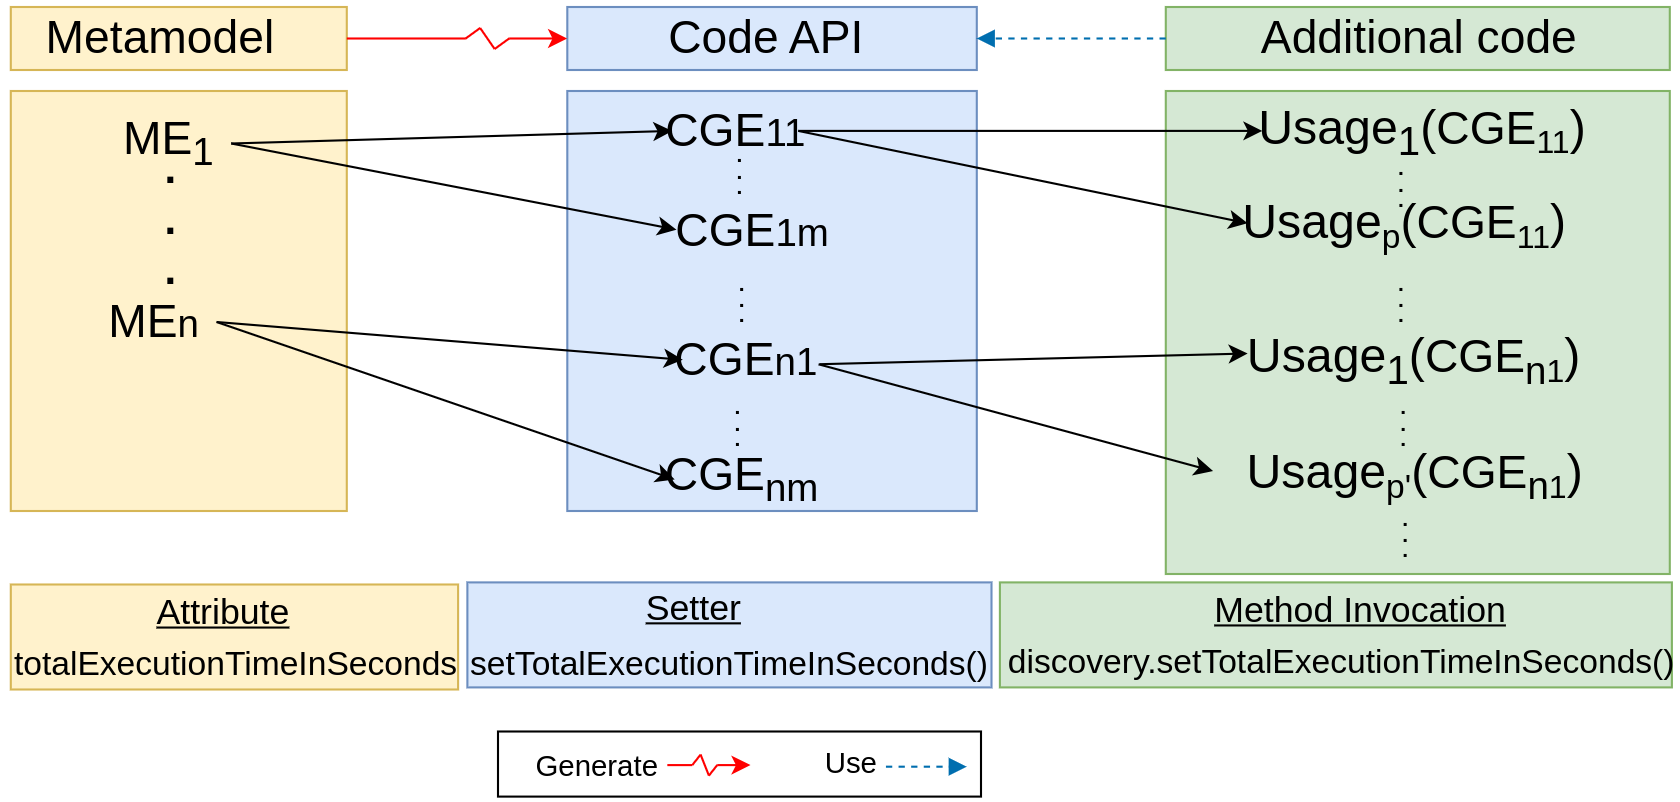
\includegraphics[width=0.5\textwidth]{pics/chapter1pics/patternusages.png}
	\caption{Schema for mapping between the metamodel and code.}
	\label{fig:patternconcept}
	\vspace{-1em}
	
\end{figure}

Algorithm \ref{algo :ErrorPatternalgo} summarizes the pattern matching process. 
Given a Java class, an error, and a list of metamodel changes, Algorithm~\ref{algo :ErrorPatternalgo} first retrieves the error AST node~{\small\boxed{line~2}}. After that, it identifies the configuration of the $GCE$ usages~{\small\boxed{Line~3}}. Then, for each metamodel change type ~{\small\boxed{lines~6,17,22,31}}, it identifies the pattern of the corresponding $GCE$ presented in Table~\ref{table:locationofMMelemen}~{\small\boxed{line~7,18,23,32}}. %the different cases of usages in the additional code~{\small\boxed{Lines~3, 2}}, \eg \emph{SimpleName}, \emph{QualifiedName}, \emph{SingleVariable}, \emph{MethodDeclaration}, etc, which are AST node types depending on its level and its position in the AST of the Java class. 
%Then, it matches it with the metamodel change causing its error~{\small\boxed{Lines ~5, 15, 18}}. This process is applied for the rest of the metamodel changes. 
%When the algorithm finds the causing change, it starts to find the 
Depending on the detected configuration, the appropriate pre-selected resolution is added to the output set~{\small\boxed{Line~10,13,19,26,35}}.
Finally, the selected resolutions set is returned for further processing in the automatic co-evolution~{\small\boxed{Line~41}}. 
Let us take the example of \texttt{"Change property type from S to T"} (last change type in Table \ref{table:ResolutionsCatalog}). It has two possible resolutions, CR16 and CR17. Assuming that we have a code error that must be co-evolved. Our pattern matching process first identifies the pattern of the corresponding $GCE_i$ from Table~\ref{table:locationofMMelemen} (Line 7), then the configuration of the $GCE_i$ usage (Lines 8). 
Algorithm \ref{algo :ErrorPatternalgo} starts by parsing the error to find the pattern of the corresponding $GCE_i$, which will help to find the causing change. The next step is to define the configuration of the $GCE_i$ which means the type of the $GCE_i$ usage. 
If it is a variable declaration (line 9), the resolution $CR16$ is returned. If any other configuration is detected, the pattern matching process returns $CR17$ as an appropriate resolution.

Note that an error can be matched with more than one resolution because a metamodel element $ME$ can be impacted by more than one change, in other terms interdependent changes. 
For example, \red{Algorithm~\ref{algo :ErrorPatternalgo} allows matching the error in~{\small\boxed{Line 17}} (rename property) and ~{\small\boxed{Line 31}} (move property) with two metamodel changes of the property \emph{totalExecutionTimeInSeconds} in Listing~\ref{lis:Modisco_Code_External_V1}.} The generated literal, which is our generated code element $GCE_i$, is used here in the configuration of a literal static field access 
\emph{\footnotesize{BenchmarkPackage.DISCOVERY\_\_TOTAL\_EXECUTION\_TIME\_IN\_SECONDS}}. The returned resolutions are $CR5$ and $CR10$~{\small\boxed{Line 19,35}}, \red{to be executed in the order of detection of their causing metamodel changes.}%\red{Empirically, we observe only the case of interdependency between a rename and move/pull/push changes.}

%Note that several patterns can be matched for a given error caused by multiple changes.
%For example, in Listing~\ref{lis:Modisco_Code_External_V1}, Algorithm~\ref{algo :ErrorPatternalgo} allows to match the error in~{\small\boxed{line 6}} with two patterns caused by the two metamodel changes rename and move of the property \emph{totalExecutionTimeInSeconds}. The generated literal, which is our generated code element $GCE_i$, used here in a static field access, 
%\emph{\footnotesize{BenchmarkPackage.DISCOVERY\_\_TOTAL\_EXECUTION\_TIME\_IN\_SECONDS}}. The matched patterns are \texttt{RenameProperty\_Literal} and \texttt{MoveProperty\_Literal}. %\texttt{RenameProperty\_ SimpleName\_Literal} and \texttt{MoveProperty\_SimpleName\_Literal}. 
%In total, we define 33 patterns that we match with the code usages and metamodel changes. We attach their list as a supplementary material\footnote{\url{https://figshare.com/s/8986914e924300be77da}}.
%Due to lack of space we attach their list as a supplementary material.



A similar mechanism is implemented for the rest of metamodel changes to select a resolution based on the pattern of $GCE_i$ and the configuration of its usage. % ~{\small\boxed{Lines 40-42}}.
For the sake of readability, Algorithm \ref{algo :ErrorPatternalgo} does not show all possible combinations of $metamodel$ $changes \times patterns \times configurations$, but few examples to illustrate its essence. \red{We nonetheless give an extended version in the appendix}

%
Finally, in our implementation, for the case of a "Delete Class" and "Delete Property", we favor the least deletion when possible. In particular, depending on the configuration usage, we select the resolution that deletes the least possible among $CR1$, $CR2$, $CR3$, $CR4$. For example, for an error in a parameter of a method call, we select the resolution $CR4$ rather than $CR1$ or $CR2$. 
In Listing \ref{lis:Modisco_Code_External_V1}, Algorithm \ref{algo :ErrorPatternalgo} matches the error in the import declaration (\textbf{Configuration}), with the deletion of the metaclass \textit{ProjectDiscovery} (\textbf{pattern}), which allows to select the resolution $CR2$.

%However, this is an implementaion strategy and could  

%For example, in Listing \ref{lis:Modisco_Code_External_V1}, the marker in {\small\boxed{line 6}}  \ie
%\texttt{BenchmarkPackage.} \emph{DISCOVERY\_\_TOTAL\_EXECUTION\_TIME\_IN\_SECONDS}  which is a static field access presents an erroneous usage of the $GCE_i$  Literal of an attribute caused by the metamodel change rename the property \emph{totalExecutionTimeInSeconds} to \emph{discoveryTimeInSeconds}. Algorithm \ref{algo :ErrorPatternalgo} allows to match it  with the pattern RenameProperty\_SimpleName\_Literal.


\definecolor{circlegreen}{HTML}{7ed321}



\begin{algorithm2e}[t]
	% \algsetup{linenosize=\tiny}
	\small
	
	\SetAlgoLined
	\KwData{javaClass, error, changesList}
	
	resolution\_s $\leftarrow \phi$ 
	
	%\While{(!usage.hasPatterns())}
	%{
		errorNode $\leftarrow$ findErrorAstNode(javaClass, error)
		
		configuration $\leftarrow$ getConfiguration(javaClass,errornode)
		
		%change $\leftarrow$ changesList.next()
		
		\For {(change  $\in$ changesList)}
		{
			\Switch{change}{
				\Case{ChangePropertyType}{
					\uIf{(match(patternGCE,change)}
					{
						
						\Switch{configuration}{
							
							\Case{VariableDeclaration}{
								
								resolution\_s.add("CR16")
							}
							
							\Other{
								
								resolution\_s.add("CR17")
							}
							
							
							
						}
					}
					
					
				}
				
				\Case{RenameProperty}{
					\uIf{(match(patternGCE,change)}
					{
						%configuration $\leftarrow$ getConfiguration(javaClass,errornode)
						
						resolution\_s.add("CR5")
						
					}
					
				}
				
				
				\Case{DeleteClass}{
					\uIf{(match(patternGCE,change)}
					{
						
						\Switch{configuration}{
							
							\Case{ImportDeclaration}{
								
								resolution\_s.add("CR2")
							}
							
							...  \emph{\textcolor{circlegreen}{/*Other configurations*/}}
							
						}
					}
				}
				
				\Case{MoveProperty}{
					\uIf{(match(patternGCE,change)}
					{
						
						\Switch{configuration}{
							
							\Case{LiteralStaticField}{
								
								resolution\_s.add("CR10")
							}
							...  \emph{\textcolor{circlegreen}{/*Other configurations*/}}    
						}
					}
					
					
				}
				\Case{... \emph{\textcolor{circlegreen}{/*Other changes*/}} }{ ... } 
				
			} 
			
			
		}
		\textbf{return} resolution\_s
		
		
		\caption{Pattern matching algorithm}
		\label{algo :ErrorPatternalgo}
	\end{algorithm2e}
	
	
	%\subsubsection{Mapping of the metamodel generated code}
	
	%\begin{comment}
	%-inputs : changes, error node
	%- analysing structure : syntactical and position in the ast refering to the different usages of metamodel element.
	%-Example
	%\end{comment}
	
	
	%\subsubsection{Pattern Detection} 
	
	%\kaouter{add concrete example using a listing : OK}
	%\DK{here take first the time to explain the table 1 of the mapping between ME types and GCE types : OK}
	%In order to add more functionalities developers enrich the generated code.  During the development process of the additional functionalities, a developer may use these generated code elements \{ $GCE_0$, $GCE_1$, ..., $GCE_n$ \}. When the developper uses a  $GCE_i$, s/he can use it in different ways, for example, an attribute literal (Table \ref{table:locationofMMelemen} ) can be used as a method declaration and method invocation parameter, and/or  as a part of a variable declaration initializer.
	%If $ME$ is changed, all the usages of  $GCE_i$ will be impacted
	%\kaouter{ Remove general example : For example if we move an attribute from a class \textit {A} to another class \textit{B} through a reference, all  the \textbf{usages} of the corresponding elements shown in the table \ref{table:locationofMMelemen} will be impacted.}
	%For example, in Listing \ref{lis:Modisco_Code_External_V1}, {\small\boxed{line 6}}, the metamodel element $ME$ that has been changed is the attribute \textit{dicoveryDate} in the class \textit{Discovery}. The corresponding generated code element $GCE$ which  is an attribute literal ( table \ref{table:locationofMMelemen}) is used as Return statement.
	
	%Two changes has been applied on this $ME$ :
	
	
	\begin{comment}[noitemsep,nolistsep]
		\item RenameProperty: dicoveryDate to discoveryDate.
		\item MoveProperty: from the class \textit{Discovery } to the class \textit{DiscoveryIteration}.
	\end{comment}
	
	%Then the usage at { \small\boxed{line 6}} is marked as an error.
	%To be able to correct a defected usage of a $GCE_i$ catched as an error, we have to find a link between the marker and the changes that caused it. The pattern matching process analyses the AST node corresponding to the marker. It finds first its AST level ( SimpleName, QualifiedName,SingleVariable, MethodDeclaration ...etc) that depends on the particular usage of the $GCE_i$. Then it analyses syntactically the AST node to link it to the right changes.
	%The second step in pattern matching is to assign a pattern to the marker. We create a data structure called \textit{Usage} that includes: The error marker, the error node, the corresponding change, and different patterns that can be associated to the error marker.
	
	%For the previous example, two patterns are detected: \textit{LiteralRename} and \textit{LiteralMove}.
	
	
	%\kaouter{here of after say that => Direct and indirect errors : \\ direct error:  the node has syntactic relation with the change element or structure relation with it,( vd in method invocation ?}
	
	%\DK{what do you mean by the "the syntactic structure of the AST node of the error and its level in the AST" ? Also, try first to explain why you need a pattern matching strategy ? like due to the variety of GCE and where they are in the code, a different  pattern of resolution can be applied ? also do you distinguish pattern and resolution or are they mixed ? : OK}
	
	
	
	\begin{comment}
		
		For example, in  marker \ref{fig:java_marker}, the detected error is about the method \textit{\texttt{setName}}, because we renamed the attribute \textit{\texttt{name}} in the class \textit{\texttt{Person}}, into \te%\\
		xtit{\texttt{familyName}}. The detected error has a \textit{\texttt{SimpleName}} corresponding node. By analyzing the structure of the node, we find that the detected pattern is \textit{\texttt{setObjectRename}}.
		
	\end{comment}
	
	
	
	
	
	
	
	\begin{comment}
		
		
		\begin{algorithm2e}[t]
			% \algsetup{linenosize=\tiny}
			\small
			
			\SetAlgoLined
			\KwData{javaClass, error, changesList}
			
			usage $\leftarrow \phi$ 
			
			%\While{(!usage.hasPatterns())}
			%{
				errorNode $\leftarrow$ findErrorAstNode(javaClass, error)
				
				%change $\leftarrow$ changesList.next()
				
				
				\uIf{(errornode.isTypeOf( SimpleName))}
				{
					\For {(change  $\in$ changesList)}
					{
						\Switch{change}{
							\Case{MoveProperty}{
								\uIf{(errornode.name="get"+change.name V errornode.name="set"+change.name)}
								{
									usage.getPatterns().
									add(UsagePattern.MoveProperty\_GetSet)
								}
								\uElseIf{(errornode.name= 
									change.className +"\_\_" +change.name)}
								{
									usage.getPatterns().
									add(UsagePattern.MoveProperty\_Literal)
								}
								\uElseIf{(errornode.name= 
									change.className +"get" +change.name)}
								{
									\uIf{(change.getUpperBound= -1)}
									{
										usage.getPatterns().
										add(UsagePattern.MoveProperty\_UpperBoundMultiple)
									}
									
									
									\uElse{
										usage.getPatterns().
										add(UsagePattern.MoveProperty\_UpperBoundSingle)
										
									}
								}
								\uElseIf{(...)}
								{
									...
								}
								
							}
							\Case{RenameProperty}{
								...
							}
							\Case{DeleteProperty}{
								...
							}
						}
					}
				} \uElseIf {( errornode.isTypeOf( QualifiedName))}
				{	  \emph{\textcolor{circlegreen}{/*repeat same matching process*/}}
					...
				}
				
				%}
			\textbf{return} usage
			
			
			\caption{Pattern matching algorithm}
			\label{algo :ErrorPatternalgo}
		\end{algorithm2e}
		
		
		\begin{table*}[t]
			\begin{tabular}{|l|l|}
				\hline
				Inputs & \begin{tabular}[c]{@{}l@{}}1) Change: move property p from class A to class B through a reference ref\\ 2) AST level : Simple Name\\ 3) Syntactic link: The identifier of the Simple Name is "get+ The name of the moved property"  \\ or  "set + The name of the moved property"\end{tabular} \\ \hline
				Output & GetorSetMoveProperty pattern                                                                                                                                                                                                                                                               \\ \hline
			\end{tabular}
			\caption{Example of GetorSetMoveProperty pattern } 
			\label{table: GetorSetMovePropertyPattern}
		\end{table*}
		
	\end{comment}
	
	\begin{algorithm2e}[t]
		% \algsetup{linenosize=\tiny}
		\small
		\SetAlgoLined
		\KwData{EcoreModelingProject, changesList}
		javaClasses $\leftarrow$ Parse(EcoreModelingProject)
		
		\For {( jc $\in$ javaClasses)}
		{
			errorsList $\leftarrow $ getErrors(jc)
			
			\While{(!errorsList.isEmpty())}
			{
				error  $\leftarrow$ errorsList.next()
				
				resolution\_s $\leftarrow$ patternMatching(jc,error, changesList)
				
				\uIf{(! resolution\_s.isEmpty()) \emph{\textcolor{circlegreen}{/*direct errors*/}}}
				{
					\For {(resolution  $\in$ resolution\_s)}
					{
						applyResolution(jc,error, resolution)
					}
				}
				\uElseIf {error.hasQuickFix() \emph{\textcolor{circlegreen}{/*indirect errors*/}}}
				%{(is\_The\_Type\_Must\_Implement\_The\_Inherited\_Abstract\_Method)}
				{
					useQuickFixes(error) %\COMMENT{Eclipse quick fix}
				}
				%\uElse {break;}
				
				refreshJavaClass(jc) 
				
				refreshErrorsList(jc, errorsList)
			}
			
		}
		
		\caption{Co-evolution of metamodel and code}
		\label{algo :overallalgo}
	\end{algorithm2e}
	
	
	
	\begin{comment}
		
		\begin{algorithm2e}[t]
			% \algsetup{linenosize=\tiny}
			\small
			\SetAlgoLined
			\KwData{EcoreModelingProject, changesList}
			javaClasses $\leftarrow$ Parse(EcoreModelingProject)
			
			\For {( jc $\in$ javaClasses)}
			{
				errorsList $\leftarrow $ getErrors(jc)
				
				\While{(!errorsList.isEmpty())}
				{
					error  $\leftarrow$ errorsList.next()
					
					usage  $\leftarrow$ matchUsagePattern(jc, error, changesList)
					
					\uIf{(! usage.getPatterns().isEmpty()) \emph{\textcolor{circlegreen}{/*direct errors*/}}}
					{
						\For {(pattern  $\in$ usage.getPatterns())}
						{
							resolution $\leftarrow$ selectResolution(pattern)
							
							applyResolution(jc, usage.getErrorNode(), resolution)
						}
					}
					\uElseIf {error.hasQuickickFix() \emph{\textcolor{circlegreen}{/*indirect errors*/}}}
					%{(is\_The\_Type\_Must\_Implement\_The\_Inherited\_Abstract\_Method)}
					{
						useQuickFixes(error) %\COMMENT{Eclipse quick fix}
					}
					%\uElse {break;}
					
					refreshJavaClass(jc) 
					
					refreshErrorsList(jc, errorsList)
				}
				
			}
			
			\caption{Co-evolution of metamodel and code}
			\label{algo :overallalgo}
		\end{algorithm2e}
		
		
		
	\end{comment}
	
	
	
	
	\subsection{Repair mechanism for the code co-evolution}
	\label{repairmechanism}
	
	
	
	After the pattern matching step, we can proceed to co-evolve the code. 
	Herein, we distinguish \textbf{direct errors} and \textbf{indirect errors}. The former are errors that do use a Generated Code Element $GCE$. They can be matched with one or many metamodel changes to select the appropriate one or many resolution(s). 
	The latter are errors that %are caused also by the metamodel evolution but they 
	do not use a generated code element. They are not matched, and hence, cannot be resolved using the pattern matching process. %They are typically errors that appear after co-evolving the direct code errors.
	
	
	
	Algorithm \ref{algo :overallalgo} presents the general process of the code co-evolution. It starts by parsing the project Java classes {\small\boxed{line~1}} to be able to access the AST of the code. Then it browses the parsed classes to retrieve the list of errors {\small\boxed{line~3}}. 
	The next step is to run the pattern matching Algorithm \ref{algo :ErrorPatternalgo} for each error to return the matched resolution(s) if any {\small\boxed{lines~4-15}}. 
	%\todo{how to avoid infinite loop?}
	%In principle, applying the resolutions require the code AST and the matched usage patterns as input to produce the co-evolved AST as output, as depicted in Figure \ref{fig:schema_resolution}.
	% of the first erroneous code usage of an evolved metamodel element. 
	%Algorithm \ref{algo :ErrorPatternalgo} first retrieves the error AST node {\small\boxed{line 5}}. Then, it matches it with the metamodel change causing its error {\small\boxed{lines 5-19}}. In particular, it covers all different code usages of the metamodel elements that are presented in Table \ref{table:locationofMMelemen}.
	%
	%\red{//explain algo 2 quickly}
	%
	%build? the first defective \textbf{usage} that we can correct {\small\boxed{line 5}}. In algorithm \ref{algo :ErrorPatternalgo}, we try to classify each marker and to detect at least one pattern for this marker. To analyse the marker, we start by retrieving the correspondant AST node { \small\boxed{line 1}}. Then depending on the type of the \textbf{ AST node} ( its level in the AST)  { \small\boxed{lines 2, 9}} and the type of the \textbf{change}  { \small\boxed{line 4}}, we can access their properties to test if there is any relation between them. In case a relation is established, a corresponding pattern is assigned  { \small\boxed{line 6}}. The usage will contain the marker, the corresponding AST node, the change, and the found patterns. 
	%
	If an error is matched with at least one resolution {\small\boxed{line~7}}, it is a \textbf{direct error}. If an error is matched with several changes {\small\boxed{lines~8-10}}, it will be resolved iteratively for each resolution{\small\boxed{lines~9}}. 
	
	In the case of an \textbf{indirect error}, we cannot apply the pattern matching process, but we still attempt to repair them with the available quick fixes in the IDE. 
	%
	%For example, \emph{unimplemented method m() of the class C} which is considered as an indirect error.\red{ It can not be matched with a metamodel pattern, because the declaration of the class C is not a code usage of the method m() (Table \ref{table:locationofMMelemen}.}, we attempt to repair it with its quick fix \emph{add the unimplemented method}.%preselected quick fix
	%
	We analyze the error message to match it with one of the proposed Java quick fixes~{\small\boxed{lines~11}}. For example, \emph{the type MC must implement the inherited abstract method} is considered as an indirect error. 
	\blue{This error can occur when a method is added in a metaclass \texttt{MC}. Classes that implement the generated interface generated from \texttt{MC} must override the new method.}
	%OLD PULL \red{This error occurs when an attribute is pulled from  a metaclass A to another metaclass B. Classes that implemented the generated interface from B must override the new methods.} 
	%\red{ It can not be matched with a metamodel pattern, because the declaration of the class C is not a code usage of the method m() (Table \ref{table:locationofMMelemen})}, w
	We attempt to repair it with its quick fix \emph{add the unimplemented method}~{\small\boxed{lines~12}}.
	
	After applying the resolutions or a quick fix, the Java class has to be refreshed. This is because the modifications of the AST will impact the list of errors and their locations in the Java class {\small\boxed{lines~13-14}}. When 
	refreshing the Java class, the list of errors typically decreases as they are co-evolved,  
	%updating the list of errors, they decrease as we co-evolve them, 
	yet, new ones may be introduced. Consequently, they will be handled in the next iterations similarly with our pattern matching and co-evolution algorithm or with the quick fixes.
	
	Finally, this process is repeated until all errors are handled. 
	However, we implemented a stopping criteria to handle the indirect errors with quick fixes. 
	It stops in two cases: 1) when only errors without any quick fix proposal remain, or 2) when the application of a quick fix causes an infinite loop \cite{cuadrado2018quick,khelladi2019detecting}, i.e., a cycle of applying a quick fix that causes a previously fixed error (A $\mapsto$ B $\mapsto$ A $\mapsto$ B $\mapsto$ ...). However, as we will see in the evaluation, these cases never happened in our executions. 
	
	%The stop condition is guaranteed because all the errors are due to metamodel changes and once an error is detected, it can be resolved using pattern matching or quick fixes.
	%\todo{say there is a risk of infinite loop between qucik fixes, and that we haev stoping cirteria for it.}  
	%Otherwise, only errors that are not matched with pattern usages and can't be resolved with quick fixes remain.
	%.all we find a defected usage that we don't know how to correct.
	
	Note that during the co-evolution process, we log the history of execution: the Java class, the error, its line, the change that provoked it, and the applied resolution(s)/quick fix in a generated report. Thus, we can generate a detailed report that allows the developer to check the modifications applied to the co-evolved code after the co-evolution is finished, i.e, their validation is not mendatory to concretly apply the resolutions.
	Table \ref{table:report} shows an example of a report for the corresponding part to our motivation example from Modisco Java Discoverer Benchmark applied co-evolution. %\red{maybe put it in 3.6?}
	
	%\red{//TODO add table of resolutions}
	
	
	%%%%%%%%%%%%%%%%%%%%%%%%%%%%%%%%%%%%%%%%%%%%%%%%%%%%%%%%%%%%%%%%%%%%%%%%%
	
	
	
	\begin{table*}[t]
		%\begin{wraptable*}{r}{5.5cm}
		\centering
		\caption{Excerpt from the traced report of Modisco Java Discoverer Benchmark project}
		\label{table:report}
		%
		%\small
		%\hspace*{-2em}
		\resizebox{17cm}{!}{
			\begin{tabular}{
					@{\hskip3pt}c@{\hskip3pt}|c@{\hskip3pt}|c@{\hskip3pt}|c@{\hskip3pt}|c@{\hskip3pt}|c@{\hskip3pt}|c@{\hskip3pt}|c@{\hskip3pt}}
				\toprule 
				File & Error& Line &Change & Resolution\\ \midrule
				\begin{tabular}[c]{@{}l@{}}CDOProjectDiscoveryImpl.java\end{tabular}
				& \begin{tabular}[c]{@{}l@{}} ProjectDiscovery \end{tabular} 
				& \begin{tabular}[c]{@{}l@{}}  29  \end{tabular} 
				&\begin{tabular}[c]{@{}l@{}}  Delete class \\ProjectDiscovery  \end{tabular}  
				&\begin{tabular}[c]{@{}l@{}}  CR2 \end{tabular}  
				
				\\ \midrule
				
				
				\begin{tabular}[c]{@{}l@{}}Report.java\end{tabular} 
				& \begin{tabular}[c]{@{}l@{}} setTotalExecutionTimeInSeconds \end{tabular}
				& \begin{tabular}[c]{@{}l@{}}  183  \end{tabular} 
				&\begin{tabular}[c]{@{}l@{}}  Rename property   \end{tabular}  
				&\begin{tabular}[c]{@{}l@{}}  CR5 \end{tabular}  
				
				\\ \midrule
				\begin{tabular}[c]{@{}l@{}}Report.java\end{tabular} 
				& \begin{tabular}[c]{@{}l@{}} setDiscoveryTimeInSeconds \end{tabular}
				& \begin{tabular}[c]{@{}l@{}}  183  \end{tabular} 
				&\begin{tabular}[c]{@{}l@{}}  Moving property  \end{tabular}  
				&\begin{tabular}[c]{@{}l@{}}  CR7  \end{tabular}  
				
				\\ \midrule
				
				\begin{tabular}[c]{@{}l@{}}CDOProjectDiscoveryImpl.java\end{tabular}
				& \begin{tabular}[c]{@{}l@{}} DISCOVERY\_\_TOTAL\_EXECUTION\_TIME\_IN\_SECONDS \end{tabular}
				& \begin{tabular}[c]{@{}l@{}}  799\end{tabular}
				&\begin{tabular}[c]{@{}l@{}}  Rename property  \end{tabular}   
				&\begin{tabular}[c]{@{}l@{}}  CR5  \end{tabular}  
				\\ \midrule
				\begin{tabular}[c]{@{}l@{}}CDOProjectDiscoveryImpl.java\end{tabular}
				& \begin{tabular}[c]{@{}l@{}} DISCOVERY\_\_DISCOVERY\_TIME\_IN\_SECONDS \end{tabular}
				& \begin{tabular}[c]{@{}l@{}}  799\end{tabular}
				&\begin{tabular}[c]{@{}l@{}}  Move property \end{tabular}   
				&\begin{tabular}[c]{@{}l@{}}  CR10\end{tabular}  
				
				\\ 
				
				
				\bottomrule
			\end{tabular}
		}
		%\end{wraptable*} 
		\vspace{-1em}
	\end{table*}
	
	%%%%%%%%%%%%%%%%%%%%%%%%%%%%%%%%%%%%%%%%%%%%%%%%%%%%%%%%%%%%%%%%%%%%%
	\begin{comment}
		
		\begin{table}[t!]
			\caption{ Patterns of usage and their corresponding resolutions.}
			\label{listofpatterns}
			\resizebox{8cm}{!} {
				\begin{tabular}{ll}
					\toprule
					Pattern of usage     & Associated resolution	 \\ \midrule		
					RenameProperty_SimpleName & CR5  \\ \midrule		
					RenameProperty_Get     & CR5  \\ \midrule		
					RenameProperty_Set    & CR5\\ \bottomrule	
					RenameProperty_Literal    & CR5\\ \bottomrule	
					RenameClass_TypeUse   & CR5\\ \bottomrule	
					RenameClass_SuperType    & CR5\\ \bottomrule	
					RenameClass_getObject    & CR5\\ \bottomrule	
					RenameClass_setObject    & CR5\\ \bottomrule	
					RenameClass_Import    & CR5\\ \bottomrule	
					RenameClass_ImportImpl    & CR5\\ \bottomrule	
					RenameClass_QualifiedType   & CR5\\ \bottomrule	
					DeleteClass_VariableDeclaration   & CR2\\ \bottomrule	
					DeleteClass_parameter    & CR1\\ \bottomrule	
					DeleteClass_parameterInMi    & CR1\\ \bottomrule	
					DeleteClass_Import    & CR2\\ \bottomrule	
					DeleteClass_MethodInvocType    & CR1\\ \bottomrule	
					DeleteClass_ClassInstance   & CR2\\ \bottomrule	
					DeleteClass_ReturnType    & CR1\\ \bottomrule	
					DeleteClass_SuperClass   & CR1\\ \bottomrule	
					DeleteClassProperty_Literal & CR4\\ \bottomrule	
					DeleteClass_ComplexStatement   & CR2\\ \bottomrule	
					DeleteClass_GetObject   & CR1\\ \bottomrule	
					DeleteProperty_MethodInvocation  & CR3\\ \bottomrule	
					MoveProperty_GetSet   &  \begin{tabular}[c]{@{}l@{}} CR7 and CR8 \\( depending on the upperBound of ref)\end{tabular}\\ \bottomrule	
					MoveProperty_MethodInvocation   & \begin{tabular}[c]{@{}l@{}} CR7 and CR8 \\( depending on the upperBound of ref)\end{tabular}   \\ \bottomrule	
					MoveProperty_MethodDeclaration  & \begin{tabular}[c]{@{}l@{}} CR7 and CR8 \\( depending on the upperBound of ref)\end{tabular}\\ \bottomrule	
					MoveProperty_Literal  & CR10\\ \bottomrule	
					PushProperty_Literal  & CR13\\ \bottomrule	
					PushProperty_GetSet  & CR11\\ \bottomrule	
					PullProperty_Literal  & CR14\\ \bottomrule	
					GeneralizeProperty_MethodInvocation   & CR6\\ \bottomrule	
					ChangeType_MethodInvocation  & CR16\\ \bottomrule	
					
				\end{tabular}
			}
		\end{table}
		%\vfill
	\end{comment}
	
	
	
	\begin{comment}
		
		\begin{algorithm}[t]
			\algsetup{linenosize=\tiny}
			\small
			\SetAlgoLined
			\KwData{cu, markersList, changesList}
			
			\For {<marker $\in$ markersList> }
			{
				usage $\leftarrow$ classify(cu,marker,changes)
				
				\uIf{(! usage.gePatterns().isEmpty())}
				{
					output $\leftarrow$  usage;
				}
			}
			output $\leftarrow$ null 
			\caption{Get first non-null usage algorithm}
			\label{algo :Usagealgo}
		\end{algorithm}
		
		
		
	\end{comment}
	
	
	
	
	
	
	
	%\subsection{Testing co-evolution}
	
	%Note that our pre-selection of a resolution may lead to a doubt about the behavioral correctness of the coevolved code. This is why we opted for the use of unit tests before and after the coevolution to check the code behavioral correctness. \todo{maybe say it in the end of 3.6 repair section, also this is part of the eval and not teh appproch, so better say it in the eval process (i think we do already)}
	
	\subsection{Prototype Implementation}
	%To be able to evaluate our approach, 
	We implemented our solution as an Eclipse Java plugin handling Ecore/EMF metamodels and their Java code. 
	
	%\red{The change detection uses EMFCompare library to compare two Ecore metamodels, the result is then formatted in our change detection interface}.
	The co-evolution process technically consists of the code AST manipulation using the JDT eclipse plugin\footnote{Eclipse Java development tools (JDT): \url{https://www.eclipse.org/jdt/core/}}.
	\begin{itemize}
		\item \textbf{Error retrieving}: there are many methods to manipulate the compilation errors of the code. We use the marker of IJavaModelMarker.JAVA\_MODEL\_PROBLEM\_MARKER. Then we filter markers whose severity value equals 2.
		\item \textbf{Change detection layer}: it consists of a set of model classes that specifies the information of each type of atomic and complex changes. 
		\item \textbf{Pattern matching}: to match the error AST node with the causing change, we proceed by string formatting between the identifier of the AST node and the relevant information encapsulated in the change. We find the corresponding configuration by looking for the higher levels of the error AST node in the code AST using the package org.eclipse.jdt.core.dom.
		\item \textbf{Resolutions} :
		The AST nodes of errors are manipulated with edit actions: modification, replacement, or deletion)  
		using the package \textit{ org.eclipse.jdt.core.dom.rewrite}, org.eclipse.text.edits.TextEdit, and \textit{org.eclipse.core.filebuffers}. 
		\item \textbf{Quick fixes} : we use \textit{org.eclipse.jdt.ui.text.java.IQuickAssistProcessor} and \textit{org.eclipse.jdt.ui.text.java.IJavaCompletionProposal}.
		
	\end{itemize}
	%To facilitate the use of our tool, we added a command the xml file of the plugin. 
	
	%The developer replaces the old version of the metamodel with the new one, and then regenerates the code API. After the regeneration step, errors will be provoked in the developer's code. He starts by selecting the path of the old and new versions of the metamodel, then he right-clicks his project, and he chooses "Coevolve the code" to run our approach. At the end of the execution, his project is coevolved and a report with the history of the execution can be found in the project's folder.
	The source code of the prototype can be found by following this link \footnote{\url{https://figshare.com/s/8986914e924300be77da}}.
	%In section \ref{repairmechanism}, we mentioned that after each resolution, we need to update the list of errors, for that, we need to save the AST after each modification  using package  \textit{org.eclipse.core.filebuffers}.
	%\red{Supplementary materials are provided\footnote{companion web page}}
	%For the metamodel changes we use an existing approach \cite{Alter2015, williams2012searching,cicchetti_managing_2009,langer_posteriori_2013,vermolen_reconstructing_2012,Khelladi2016}. 
	
	%\todo{here say that we generate a report linking mm changes, to impacted lines in the code, error message, matched pattern, and how they were co-evoved it which resoluton}